\documentclass{article}
\usepackage[final]{neurips_2020}
\usepackage[utf8]{inputenc}
\usepackage{ctex}
\usepackage[T1]{fontenc}
\usepackage{hyperref}
\usepackage{url}
\usepackage{booktabs}
\usepackage{algorithm}
\usepackage{algpseudocode}  % 这个包用于算法伪代码

\usepackage{amsfonts}
\usepackage{amsmath}
\usepackage{nicefrac}
\usepackage{microtype}
\usepackage{indentfirst}
\usepackage{listings}
\usepackage{graphicx}
\usepackage{float}

\usepackage[dvipsnames]{xcolor}
\lstset{
    language=Python,
    basicstyle=\ttfamily,
    breaklines=true,
    keywordstyle=\bfseries\color{NavyBlue},
    morekeywords={},
    emph={self},
    emphstyle=\bfseries\color{Rhodamine},
    commentstyle=\itshape\color{black!50!white},
    stringstyle=\bfseries\color{PineGreen!90!black},
    columns=flexible,
    numbers=left,
    numbersep=2em,
    numberstyle=\footnotesize,
    frame=single,
    framesep=1em,
    showstringspaces=false
}
\setlength{\parindent}{2em}

\title{中山大学计算机院本科生实验报告\\
    (2024学年秋季学期)}

\begin{document}
\maketitle
课程名称:强化学习与博弈论 \qquad\qquad\qquad\qquad\qquad\qquad
批改人:
\begin{table*}[h]
    \centering
    \begin{tabular}{|c|c|c|c|} \hline
        实验    & Assignment1                 & 专业(方向) & 计算机科学与技术 计科一班 \\ \hline
        学号    & 21307099                           & 姓名     & 李英骏           \\\hline
        Email & \texttt{liyj323@mail2.sysu.edu.cn} & 完成日期   & \today        \\\hline
    \end{tabular}
\end{table*}
\tableofcontents

\newpage
\section{实验目的}
Solve the Maze Problem using Value Iteration. Code has already been uploaded to \href{https://github.com/KFCCrazzzyThursday/rl_and_game_theory/blob/main/MDP.cpp}{GitHub}


\section{实验过程和核心代码}
\subsection{MDP definition}
\begin{itemize}
    \item $\mathcal{S}$: 迷宫中的所有可行走位置。
    \item $\mathcal{A}$: NESW四个方向。
    \item $\mathcal{P}$: 动作导致的状态转移是确定性的。
    \item $\mathcal{R}$ : 每一步的奖励为 -1。
    \item $\gamma$: 设为 1.0, 因为我们希望最小化步数(总惩罚)。
\end{itemize}
即代码如下部分:
\begin{figure}[H]
    \centering
    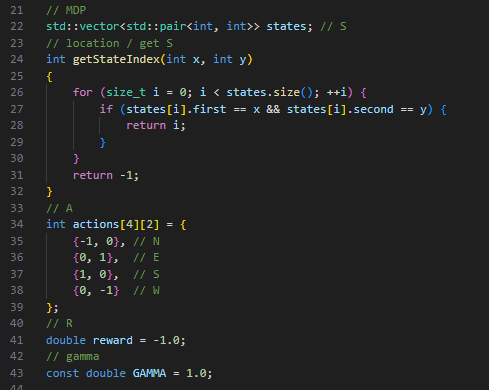
\includegraphics[width=0.7\linewidth]{./image/image4.png}
    \caption{}
\end{figure}

\subsection{价值迭代算法}
价值迭代算法是一种动态规划算法,用于求解MDP的最优策略。其核心思想是通过迭代地更新每个状态的价值函数,直到收敛到最优价值函数,然后从中导出最优策略。

\subsubsection{价值函数}
\begin{itemize}
    \item 状态价值函数($V$):表示在状态 $s$ 下,按照最优策略所能获得的期望累积奖励。
    \item 动作价值函数($Q$):表示在状态 $s$ 下,采取动作 $a$,然后按照最优策略所能获得的期望累积奖励。
\end{itemize}

\subsubsection{Bellman 最优方程}
价值迭代算法基于 Bellman 最优方程:

\[
V(s) = \max_{a \in A(s)} \left[ R(s, a) + \gamma \sum_{s'} P(s' | s, a) V(s') \right]
\]

其中:
\begin{itemize}
    \item $V(s)$:状态 $s$ 的价值。
    \item $R(s, a)$:在状态 $s$ 下采取动作 $a$ 获得的即时奖励。
    \item $\gamma$:折扣因子。
    \item $P(s' | s, a)$:从状态 $s$ 采取动作 $a$ 转移到状态 $s'$ 的概率。
    \item $V(s')$:下一状态 $s'$ 的价值。
\end{itemize}

\subsubsection{算法步骤}

\begin{algorithm}[H]
    \caption{价值迭代算法}
    \begin{algorithmic}[1]
        \State Initialize $V(s)$ for all states $s$
        \Repeat
            \State $\Delta \gets 0$
            \For{each state $s$}
                \State $v \gets V(s)$
                \State $V(s) \gets \max_{a \in A(s)} \left[ R(s, a) + \gamma \sum_{s'} P(s' | s, a) V(s') \right]$
                \State $\Delta \gets \max(\Delta, |v - V(s)|)$
            \EndFor
        \Until{$\Delta < \theta$}
    \end{algorithmic}
\end{algorithm}
对应代码的如下部分:
\begin{figure}[H]
    \centering
    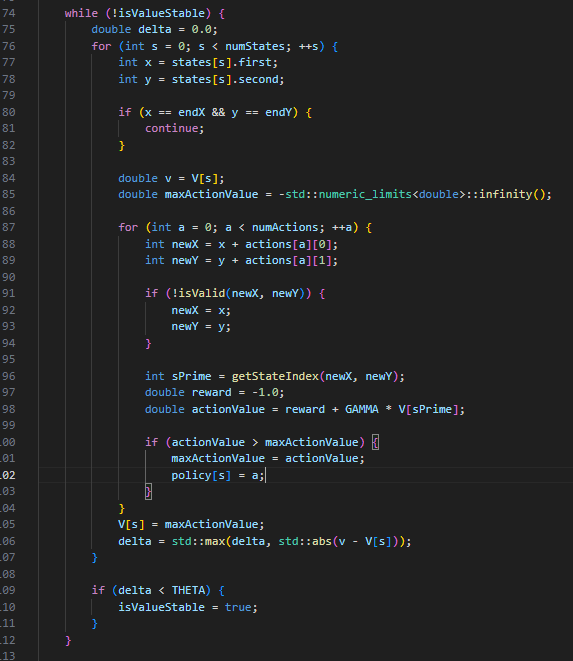
\includegraphics[width=0.8\linewidth]{./image/image1.png}
    \caption{}
\end{figure}

\section{实验结果}
\begin{figure}[H]
    \centering
    \begin{minipage}{0.35\linewidth}
        \centering
        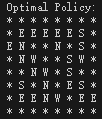
\includegraphics[width=\linewidth]{./image/image3.png}
        \caption{输出}
    \end{minipage}
    \hspace{0.05\linewidth} % 调整图间距
    \begin{minipage}{0.35\linewidth}
        \centering
        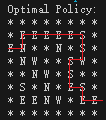
\includegraphics[width=\linewidth]{./image/image2.png}
        \caption{规划路线}
    \end{minipage}
\end{figure}

\section{实验感想}
在本次实验中,我深入了解了强化学习中的价值迭代算法及其在迷宫问题中的应用。通过将理论知识与实践相结合,我不仅掌握了如何定义马尔可夫决策过程(MDP),还实践了价值迭代算法的实现。这种算法通过不断更新状态价值函数,最终收敛到最优策略,反映了动态规划在强化学习中的重要性。

\end{document}
